\documentclass[12 pt]{article}
\usepackage[left=2.66cm,top=3cm,right=2.66cm,bottom=3cm,bindingoffset=0.5cm]{geometry}

\usepackage{graphicx}
\usepackage{setspace}
\usepackage{enumitem}
\onehalfspacing

\begin{document}
\begin{titlepage}
\begin{Huge}
\begin{center}
\textsc{ RSA Algorithm \linebreak
and \linebreak
Public Key Cryptosystems}
\end{center}
\end{Huge}
\begin{center}
\begin{large}
\textsl{ Rohan Datta, Divya Raj}
\end{large}
\end{center}

\bigskip 
\begin{center}
\textbf{Abstract}
\end{center}
This text discusses the concept behind public key cryptosystems, while focusing on a very popular encryption method. It also presents an array of real world implementations of the algorithm.
Building upon ground-breaking research papers, it interprets the intriguing subject matter into an accessible form, and goes further to put forth their major applications and a few of their limitless possibilities.
\\
\\
\textit{Key words and phrases:} cryptosystems, discrete mathematics, encryption, decryption, prime numbers, digital signatures, public key cryptosystems, authentication, cyber security.
\end{titlepage}
\pagebreak
\begin{LARGE}	
\begin{center}
\textbf{\textsc{Introduction to Public-Key Cryptography}}
\end{center}
\end{LARGE}

\noindent 
\\Public key cryptography, or asymmetrical cryptography, is any cryptographic system that uses pairs of keys: public keys which may be disseminated widely, and private keys which are known only to the owner. This accomplishes two functions: authentication, which is when the public key is used to verify that a holder of the paired private key sent the message, and encryption, whereby only the holder of the paired private key can decrypt the message encrypted with the public key.
\\\\The various methods that can and were used as alternatives to the public key systems are as follows:
\\\textbf{1. Symmetric}\\In a symmetric-key algorithm, both the sender and receiver share the key. The sender uses the key to hide the message. Then, the receiver will use the same key in the opposite way to reveal the message. For centuries, most cryptography has been symmetric. The problem with this system is that you have to make sure that the key is shared in a secure way, thus creating a chicken - egg problem.

\begin{figure}[h!]
  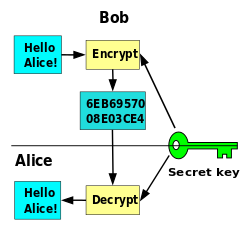
\includegraphics[width=60mm]{Symmetric_key_encryption.png}
  \centering
  \caption{Symmetric-key cryptography.}
  \label{fig:Symmetric-key cryptography}
\end{figure}
\noindent
\\\textbf{2. Decryption - Encryption in the middle}
\\In this system instead of having just two parties like above, one common third party(mostly a server) is added. So now, the sender and the server share a key(say K\textsubscript{a}), and the server and the receiver share a key(say K\textsubscript{b}). The sender's message is encrypted using K\textsubscript{a}, is decrypted at the server, then it is encrypted by K\textsubscript{b}, and sent to the receiver, where it finally gets decrypted and the message is delivered. The problem here is that the server becomes an obvious fail point, if its security is compromised, the whole system might fail.

\textbf{Hence the Public-Key system}, which is as follows:
\\In a public key encryption system, any person can encrypt a message using the public key of the receiver, but such a message can be decrypted only with the receiver's private key. For this to work it must be computationally easy for a user to generate a public and private key-pair to be used for encryption and decryption.

\begin{figure}[h!]
  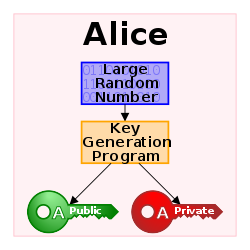
\includegraphics[width=50mm]{250px-Public-key-crypto-1.png}
  \centering
  \caption{A typically large and random number is used to begin generation of an acceptable pair of keys suitable for use by an asymmetric key algorithm.}
  \label{fig:PublicKey-NumGen}
\end{figure}

The strength of a public key cryptography system relies on the degree of difficulty (computational impracticality) for a properly generated private key to be determined from its corresponding public key. Security then depends only on keeping the private key private, and the public key may be published without compromising security.


\begin{figure}[h!]
  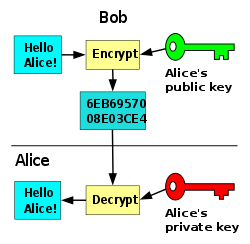
\includegraphics[width=50mm]{250px-Public_key_encryption.png}
  \centering
  \caption{The basic mechanism of a public key encryption system.}
  \label{fig:PublicKey-Basic}
\end{figure}

Public key cryptography systems often rely on cryptographic algorithms based on mathematical problems that currently admit no efficient solution — particularly those inherent in certain integer factorization, discrete logarithm, and elliptic curve relationships. Public key algorithms, unlike symmetric key algorithms, do not require a secure channel for the initial exchange of one (or more) secret keys between the parties.

Because of the computational complexity of asymmetric encryption, it is usually used only for small blocks of data, typically the transfer of a symmetric encryption key (e.g. a session key). This symmetric key is then used to encrypt the rest of the potentially long message sequence. The symmetric encryption/decryption is based on simpler algorithms and is much faster.

\noindent
Two of the best-known uses of public key cryptography are:

\textbf{1. }Public key encryption, in which a message is encrypted with a recipient's public key. The message cannot be decrypted by anyone who does not possess the matching private key, who is thus presumed to be the owner of that key and the person associated with the public key. This is used in an attempt to ensure confidentiality.

An analogy to public key encryption is that of a locked mail box with a mail slot. The mail slot is exposed and accessible to the public – its location (the street address) is, in essence, the public key. Anyone knowing the street address can go to the door and drop a written message through the slot. However, only the person who possesses the key can open the mailbox and read the message.

\textbf{2. }Digital signatures, in which a message is signed with the sender's private key and can be verified by anyone who has access to the sender's public key. This verification proves that the sender had access to the private key, and therefore is likely to be the person associated with the public key. This also ensures that the message has not been tampered with, as a signature is mathematically bound to the message it originally was made with, and verification will fail for practically any other message, no matter how similar to the original message.

An analogy for digital signatures is the sealing of an envelope with a personal wax seal. The message can be opened by anyone, but the presence of the unique seal authenticates the sender.

\pagebreak

\begin{Large}
\noindent \textbf{{Uses of Public-key Cryptography}}
\end{Large}
\\Public key cryptography is often used to secure electronic communication over an open networked environment such as the Internet, without relying on a hidden or covert channel, even for key exchange. Open networked environments are susceptible to a variety of communication security problems, such as man-in-the-middle attacks and spoofs. Communication security typically includes requirements that the communication must not be readable during transit (preserving confidentiality), the communication must not be modified during transit (preserving the integrity of the communication), the communication must originate from an identified party (sender authenticity), and the recipient must not be able to repudiate or deny receiving the communication. Combining public key cryptography with an Enveloped Public Key Encryption (EPKE) method, allows for the secure sending of a communication over an open networked environment. In other words, even if an adversary listens to an entire conversation including the key exchange, the adversary would not be able to interpret the conversation.

\pagebreak

\begin{LARGE}
\begin{center}
  \textbf{{RSA Algorithm}}
\end{center}
\end{LARGE}\bigskip

\noindent RSA algorithm is an asymmetric cryptographic algorithm that is used extensively by computers nowadays. It was proposed by Ron Rivest, Adi Shamir and Leonard Adleman in their 1978 paper [reference], and hence, bears their name. It is one of the most popular implementations of public key cryptosystems.\bigskip

\noindent It is driven by the fact that finding the prime factors of a number is one of the most complex mathematical problems. Initially, the user creates and publishes the product of two large prime numbers, along with an auxiliary value. The auxiliary value takes up the role of the ``public key'' which is known to all. \emph{But, the prime factors must be kept secret.}\bigskip

1. Choose\ two\ different,\ large,\ random\  prime\  numbers\ \textbf{p} and \textbf{q}

2. Calculate \textbf{n} = \textbf{p}*\textbf{q}

3. \textbf{\boldmath $\phi(n)$ = (p - 1)*(q - 1)}

4. Choose an integer \textbf{e} such that:

\begin{itemize} \setlength\itemsep{1 em}
\setstretch{0.61803398875} \item  1 \textless \textbf{e} \textless \boldmath$\phi(n)$
\setstretch{0.61803398875} \item \textbf{e} is co-prime to \boldmath$\phi(n)$
\end{itemize}

5. Compute \textbf{d} such that \boldmath \textbf{d}*\textbf{e} = 1+\textbf{k}*\boldmath $\phi(n)$
\bigskip
\\
A popular choice for public exponents is \textbf{e} = $2$ \textsuperscript{$16$}+$1$

\end{document}


